\begin{figure}
  \centering
  \captionsetup{justification=centering}
  \begin{subfigure}[b]{0.4\linewidth}
    \label{subfig:top_view}
    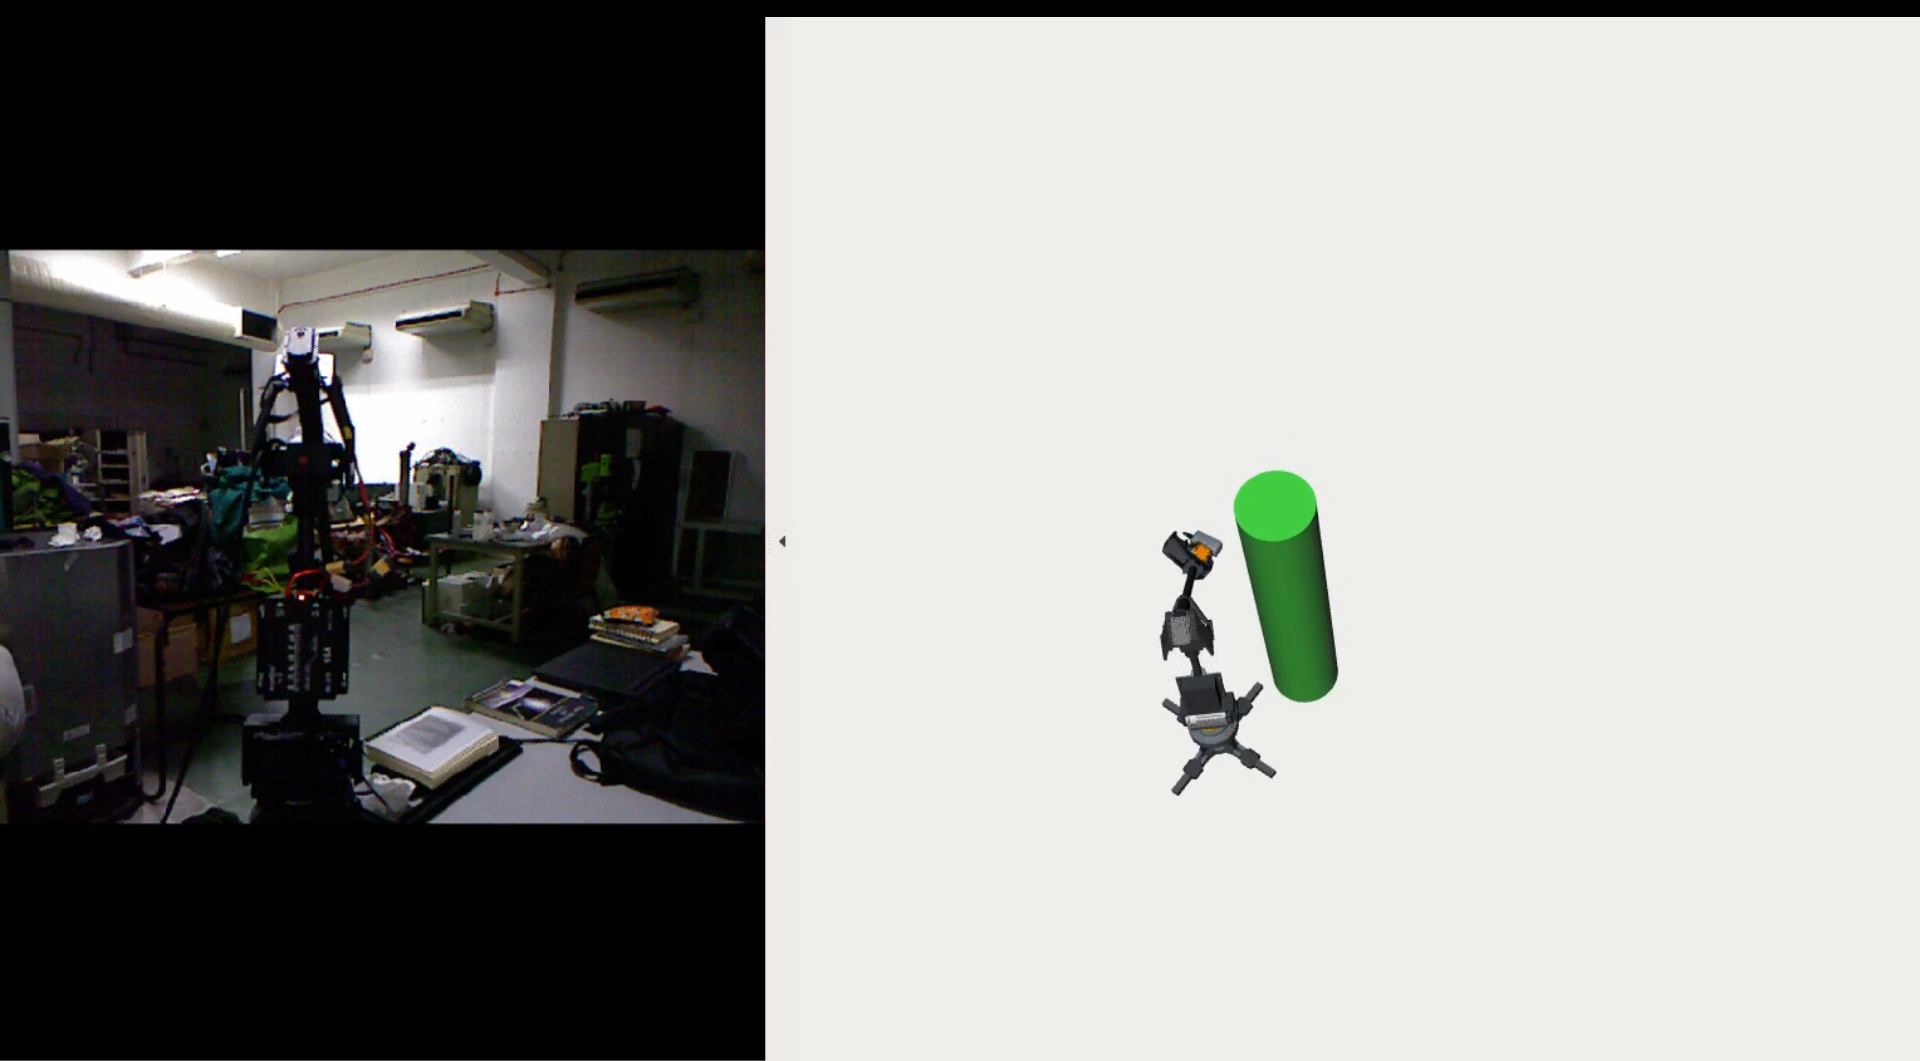
\includegraphics[width=\linewidth]{obs_avoidance1.png}
     \caption{}
  \end{subfigure}
  \begin{subfigure}[b]{0.4\linewidth}
    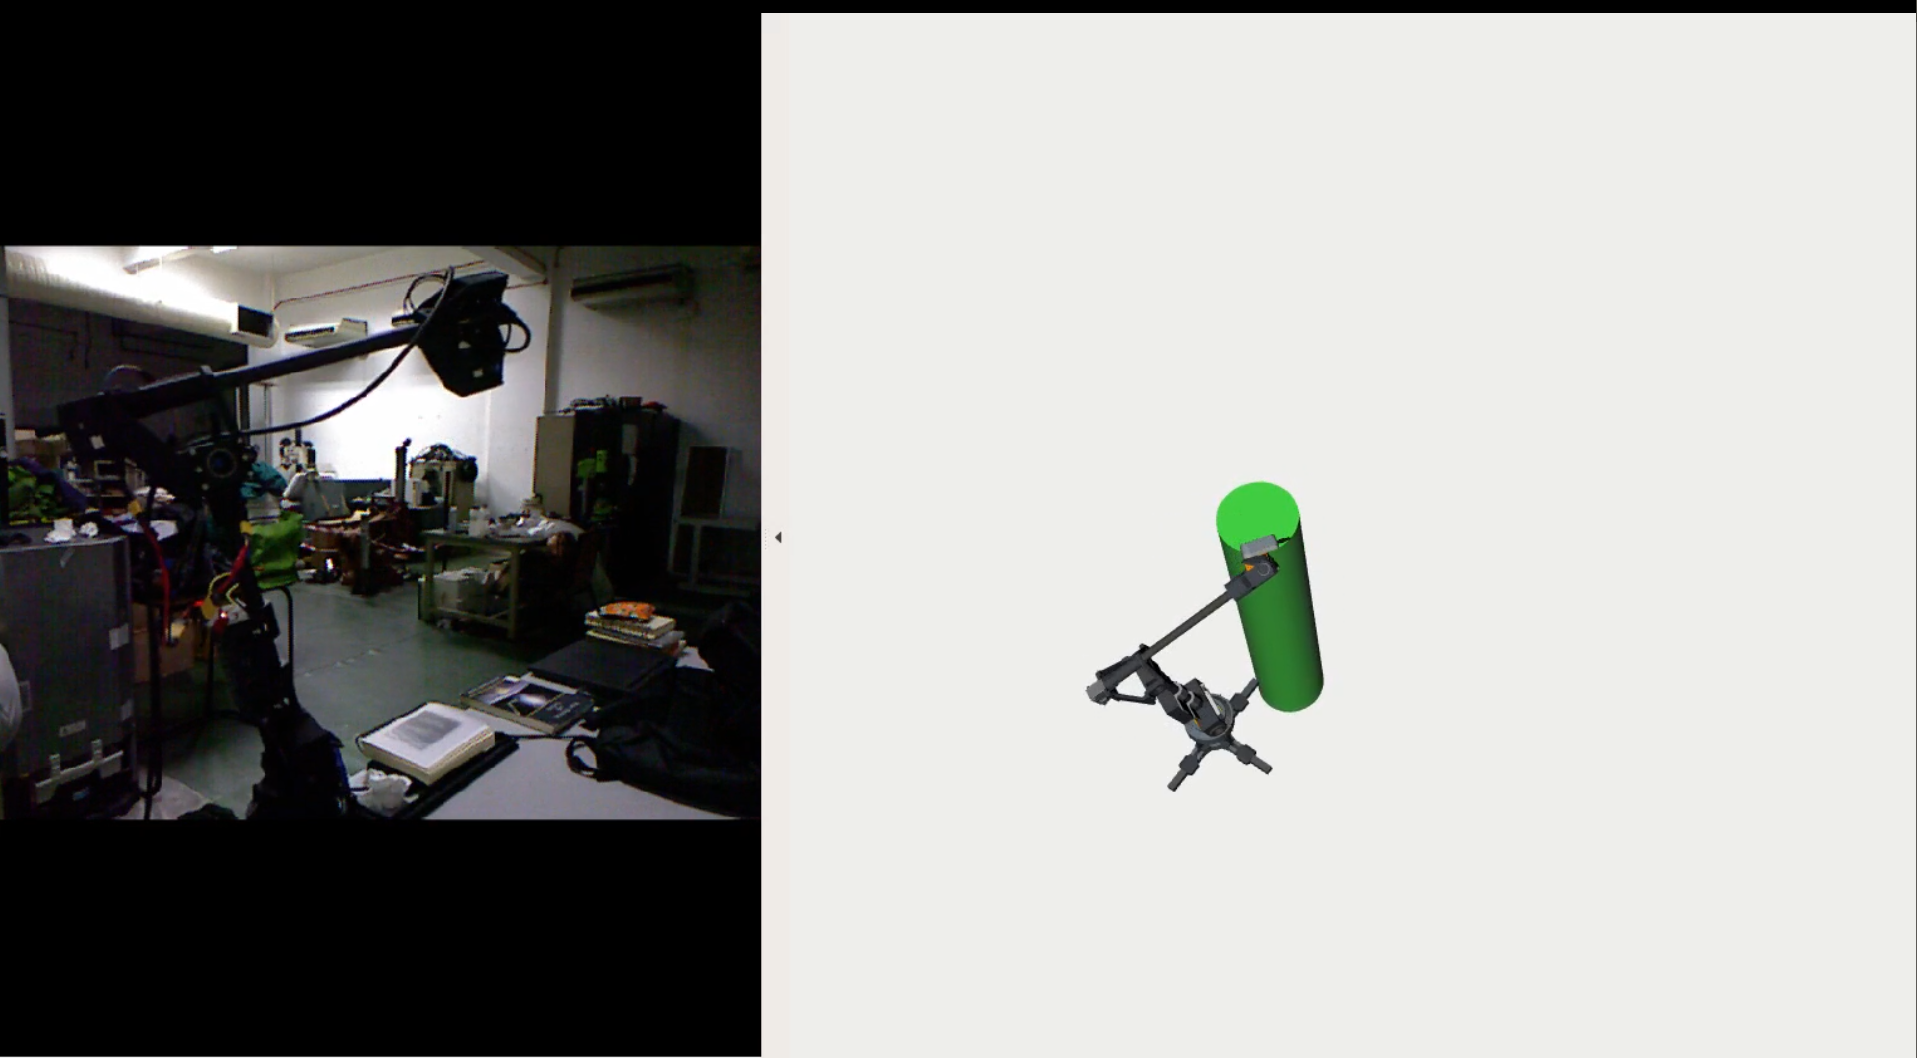
\includegraphics[width=\linewidth]{obs_avoidance2.png}
    \caption{}
  \end{subfigure}
  \begin{subfigure}[b]{0.4\linewidth}
    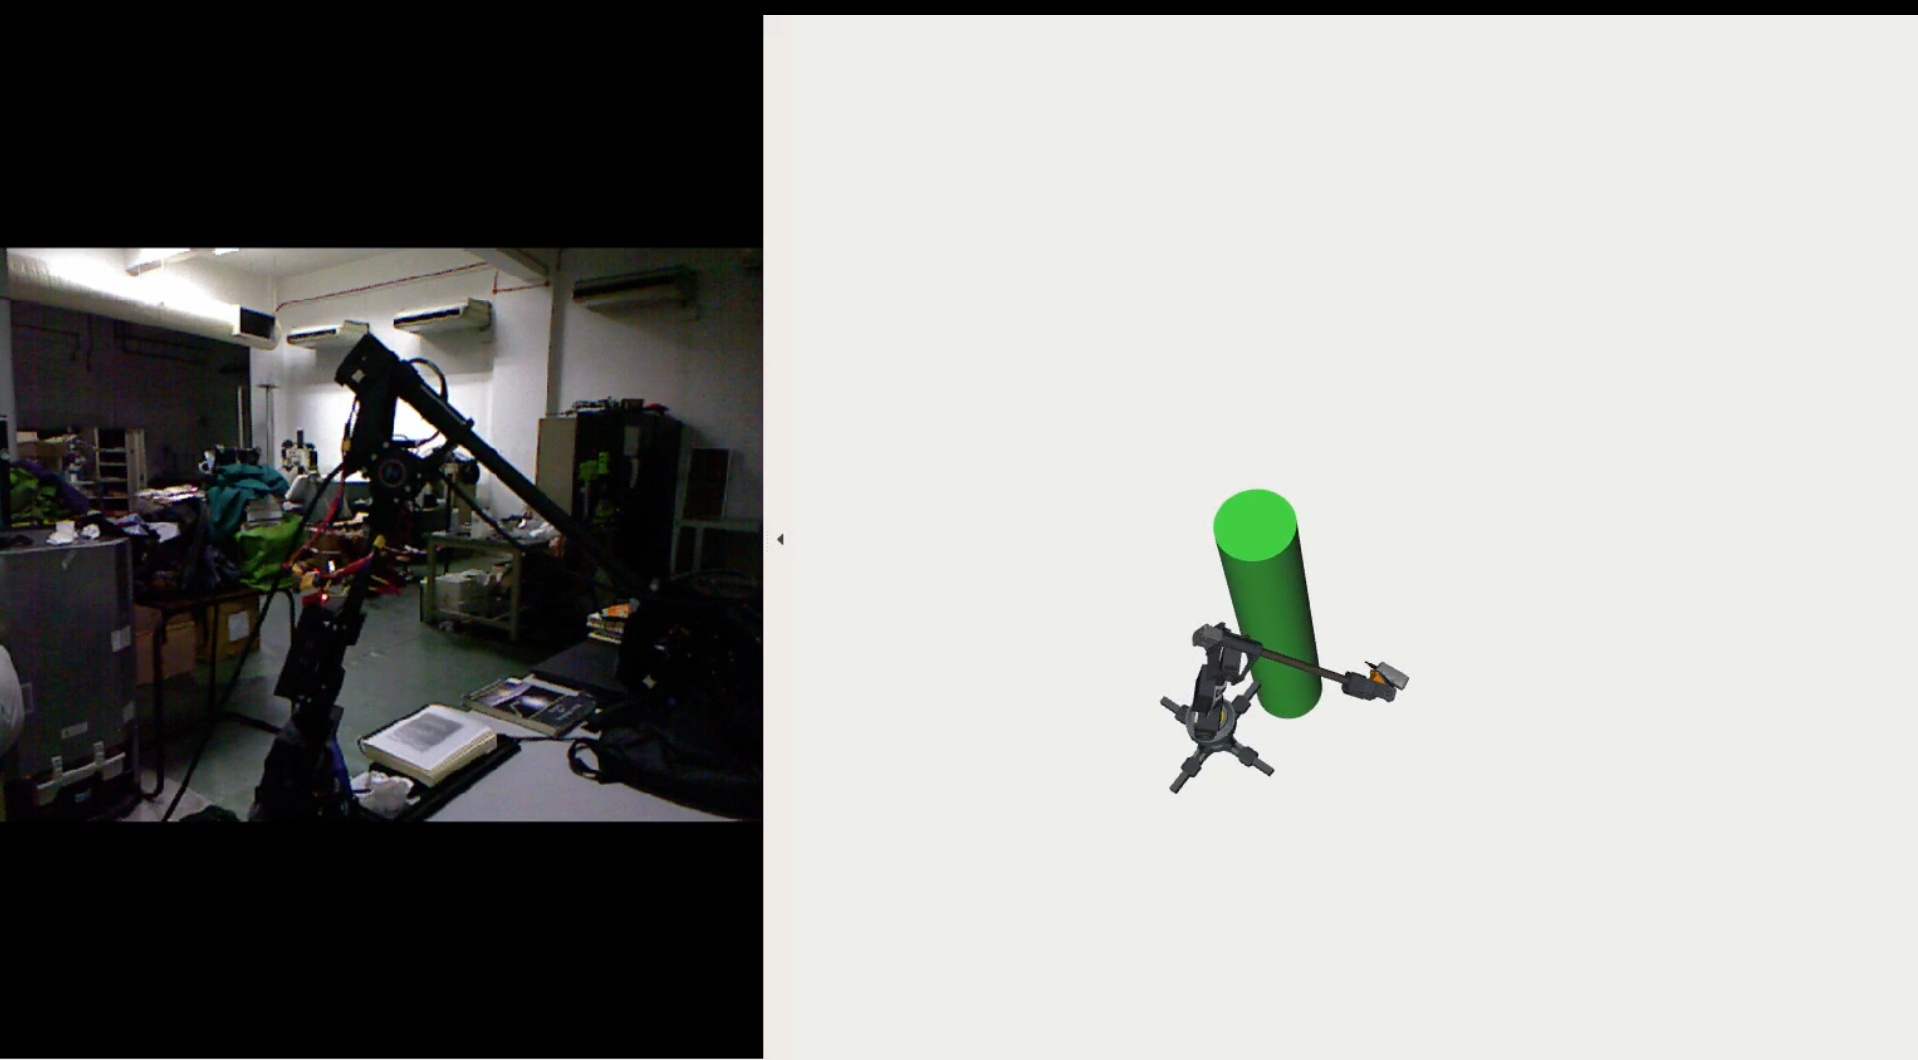
\includegraphics[width=\linewidth]{obs_avoidance3.png}
    \caption{}
  \end{subfigure}
  \begin{subfigure}[b]{0.4\linewidth}
    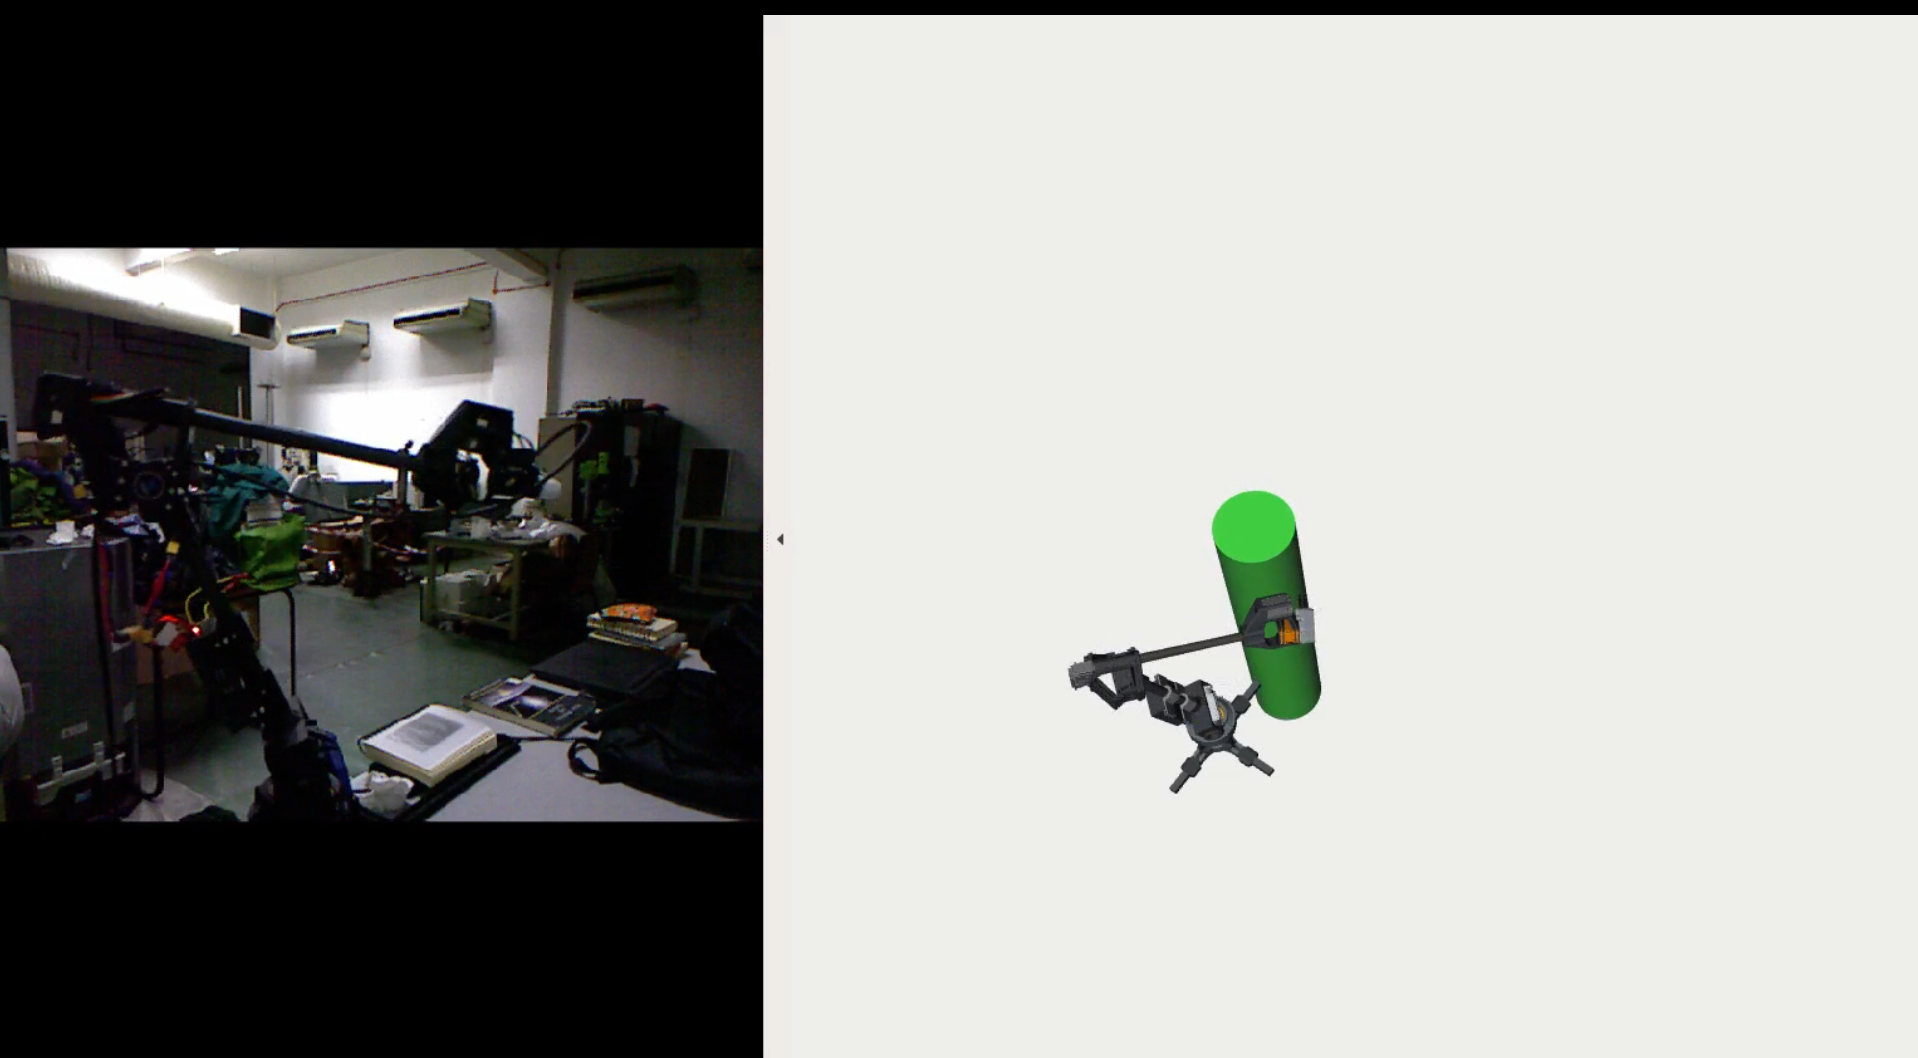
\includegraphics[width=\linewidth]{obs_avoidance4.png}
    \caption{}
  \end{subfigure}
  \begin{subfigure}[b]{0.4\linewidth}
    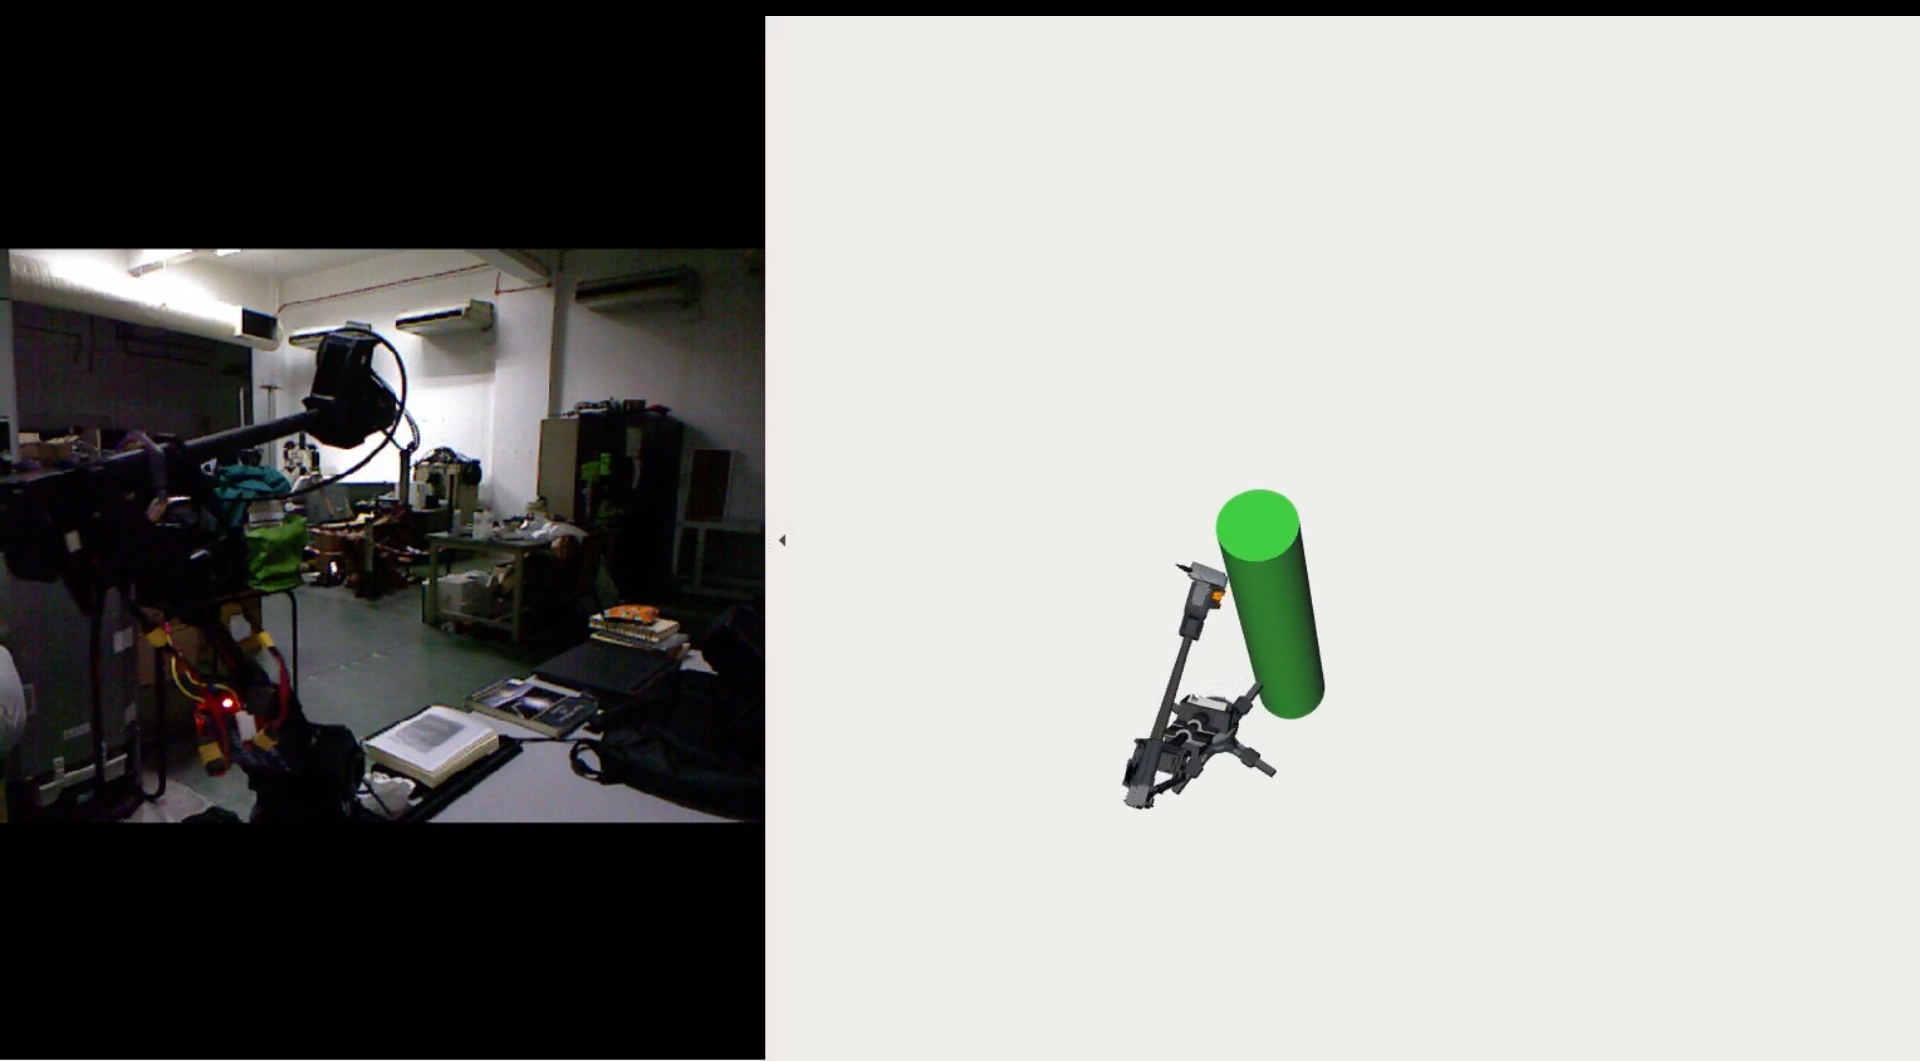
\includegraphics[width=\linewidth]{obs_avoidance5.png}
    \caption{}
  \end{subfigure}
  \begin{subfigure}[b]{0.4\linewidth}
    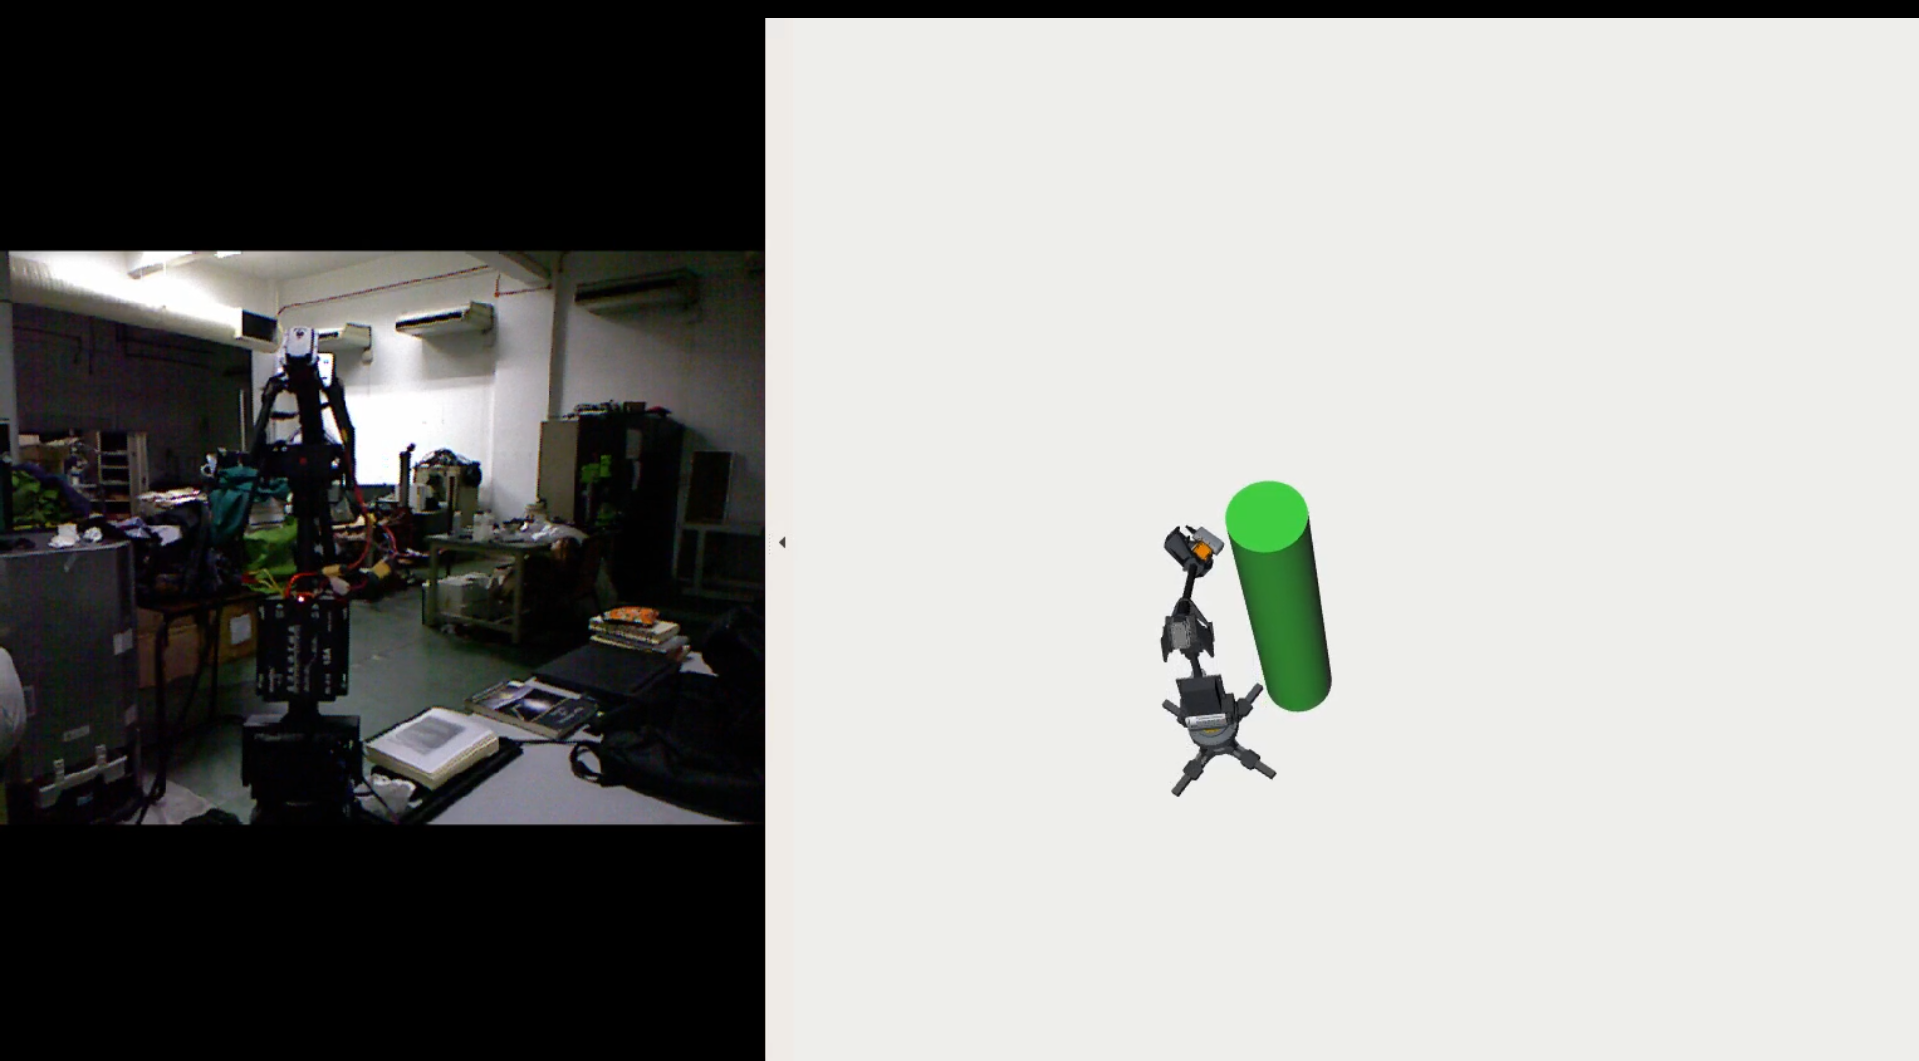
\includegraphics[width=\linewidth]{obs_avoidance6.png}
    \caption{}
  \end{subfigure}

  \caption{The sequence of motion when \rimini~ successfully avoid a moving obstacle
  when the obstacles at a turning point to move away from the hardware.}
  \label{fig:obs_avoidance}
\end{figure}
